\documentclass[openright,usenames,dvipsnames]{abnt/normas-utf-tex} %openright = o capitulo comeca sempre em paginas impares
%\documentclass[oneside]{normas-utf-tex} %oneside = para dissertacoes com numero de paginas menor que 100 (apenas frente da folha) 


% ---
% Pacotes fundamentais 
% ---
\usepackage[brazil]{babel} % pacote portugues brasileiro
\usepackage[utf8]{inputenc} % pacote para acentuacao direta
\usepackage{amsmath,amsfonts,amssymb} % pacote matematico
\usepackage{graphicx} % pacote grafico
\usepackage{times} % fonte times
\usepackage[final]{pdfpages} % adicao da ata
\usepackage{indentfirst}
\usepackage{geometry}
\usepackage{diagbox}
\usepackage{adjustbox}
\usepackage{booktabs}
\usepackage{longtable, ltcaption}
\usepackage{slashbox}
\usepackage{rotating}
\usepackage{enumitem}
\usepackage{ragged2e}
\usepackage{pdflscape}
\usepackage{afterpage}
\usepackage{chronology}
\usepackage[colorinlistoftodos]{todonotes}
\usepackage{verbatim}
\usepackage{pgfgantt}
\usepackage{tikz}
\usetikzlibrary{mindmap,trees}
\usepackage[edges]{forest}
\usetikzlibrary{fit}
\usetikzlibrary{shapes,backgrounds}
\usetikzlibrary{arrows.meta}
\pgfdeclarelayer{background}
\pgfdeclarelayer{foreground}
\pgfsetlayers{background,main,foreground}
\usepackage{pgfplots}
\usepackage{multirow}
\usepackage{float}
\usepackage{placeins}
\usepackage{caption}
 \captionsetup[longtable]{labelfont=bf,textfont=normalfont,textfont=bf}
\usepackage{acronym}
\usepackage{lipsum}
% ---
% Pacotes de citações
% ---

\usepackage[alf,abnt-emphasize=bf,bibjustif,recuo=0cm, abnt-etal-cite=2, abnt-etal-list=99]{abnt/abntex2cite} %configuracao correta das referencias bibliograficas.
% force A4 paper format


\special{papersize=210mm,297mm}

\usepackage{lipsum}
\geometry{left=3.0cm,right=2cm,top=3cm,bottom=2cm} 

\setlength{\parindent}{1.25cm}

\graphicspath{ {figuras/} }

\ganttset{group/.append style={Dandelion},
	milestone/.append style={BrickRed},
	progress label node anchor/.append style={text=red}}

\tikzset{%
  >={Latex[width=2mm,length=2mm]},
  % Specifications for style of nodes:
            rec/.style = {rectangle, rounded corners, draw=black, minimum width=4cm, minimum height=1cm,  text centered, font=\sffamily, fill=blue!30},
             rec1/.style = {rectangle, rounded corners, draw=black, minimum width=4cm, minimum height=1.5cm, text width=3.8cm,  text centered, font=\sffamily, fill=blue!30},
            rec2/.style = {rectangle, rounded corners, draw=black, minimum width=4cm, minimum height=2cm,   text centered, font=\sffamily, fill=blue!30},
             rec3/.style = {rectangle, rounded corners, draw=black, minimum width=4cm, minimum height=5cm,   text centered, font=\sffamily, fill=blue!30},
              rec4/.style = {rectangle, rounded corners, draw=black, minimum width=4cm, minimum height=.5cm,   text centered, font=\sffamily, fill=blue!30},
 tri/.style = {isosceles triangle,draw,inner sep=0pt,anchor=south,shape border rotate=90,isosceles triangle stretches, fill=red!30}
    }

% ---
% Informações de dados para CAPA e FOLHA DE ROSTO
% ---
\instituicao{UNIVERSIDADE TECNOLÓGICA FEDERAL DO PARANÁ} % nome da instituicao
\programa{PROGRAMA DE PÓS-GRADUAÇÃO EM ENGENHARIA MECÂNICA E DE MATERIAIS} % nome do programa
\area{Engenharia de Manufatura} % 

\documento{Dissertação} % [Dissertação] ou [Tese]
\nivel{Mestrado} % [Mestrado] ou [Doutorado]
\titulacao{Mestre} % [Mestre] ou [Doutor]

\titulo{\MakeUppercase{Título para a Tese ou Dissertação}} % titulo do trabalho em portugues
\title{\MakeUppercase{Title for Thesis or Dissertation}}
\autor{Seu nome completo} % autor do trabalho
\cita{Colocar modo de citar seu nome} % sobrenome (maiusculas), nome do autor do trabalho

\palavraschave{Palavra-chave 1; Palavra-chave 2; ...; Palavra-chave n} % palavras-chave do trabalho
\keywords{Keywords 1; Keywords 2; ...; Keywords n} % palavras-chave do trabalho em ingles
\local{Curitiba}
\data{2018}

\orientador{Nome do orientador} % nome do orientador do trabalho
%\orientador[Orientadora:]{Nome da Orientadora} % <- no caso de orientadora, usar esta sintaxe
%\coorientador{Nome do Co-orientador} % nome do co-orientador do trabalho, caso exista
%\coorientador[Co-orientadora:]{Nome da Co-orientadora} % <- no caso de co-orientadora, usar esta sintaxe
%\coorientador[Co-orientadores:]{Nome do Co-orientador} % no caso de 2 co-orientadores, usar esta sintaxe
%\coorientadorb{Nome do Co-orientador 2}	% este comando inclui o nome do 2o co-orientador



\comentario{\UTFPRdocumentodata\ apresentada ao \UTFPRprogramadata\ da \ABNTinstituicaodata\, como requisito parcial para obtenção do título de \UTFPRtitulacaodata\ em Engenharia Mecânica – Área de concentração: \UTFPRareadata.}
% ---

%Lista de abreviaturas



%\include{pretextuais/listadesiglas}

% desativa hifenizacao mantendo o texto justificado.
% thanks to Emilio C. G. Wille
\tolerance=1
\emergencystretch=\maxdimen
\hyphenpenalty=10000
\hbadness=10000
\sloppy

%---------- Inicio do Documento ----------
\begin{document}
\renewcommand\LTcaptype{quadro}
\pgfdeclarelayer{background}
\pgfdeclarelayer{foreground}
\pgfsetlayers{background,main,foreground}
%%%%%%%%%%%%%%%%%%%%%%%%%%%%%%%%%%%%%%%%%%%%%%%%%%%% ELEMENTOS  PRETEXTUAIS
%%%%%%%%%%%%%%%%%%%%%%%%%%%%%%%%%%%%%%%%%%%%

\capa % geracao automatica da capa
\folhaderosto % geracao automatica da folha de rosto

% Lembre-se de que a ficha catalografica eh impressa no verso da folha de rosto
% Ficha catalografica
%\fichacatpum{T137} %preencher conforme modelo recebido pela biblioteca
%\fichacatautor{\UTFPRcitadata}
%\fichacatpgbib{\pageref{bibstart}-\pageref{bibend}}
%\fichacatpalcha{\UTFPRpalavraschavedata}
%\fichacatpdois{CDD (22. ed.) 621.3}
%\fichacatbib{Biblioteca xxxxxx} %preencher conforme modelo encaminhado pela bibliotecária
%\fichacat

% insercao da ATA
%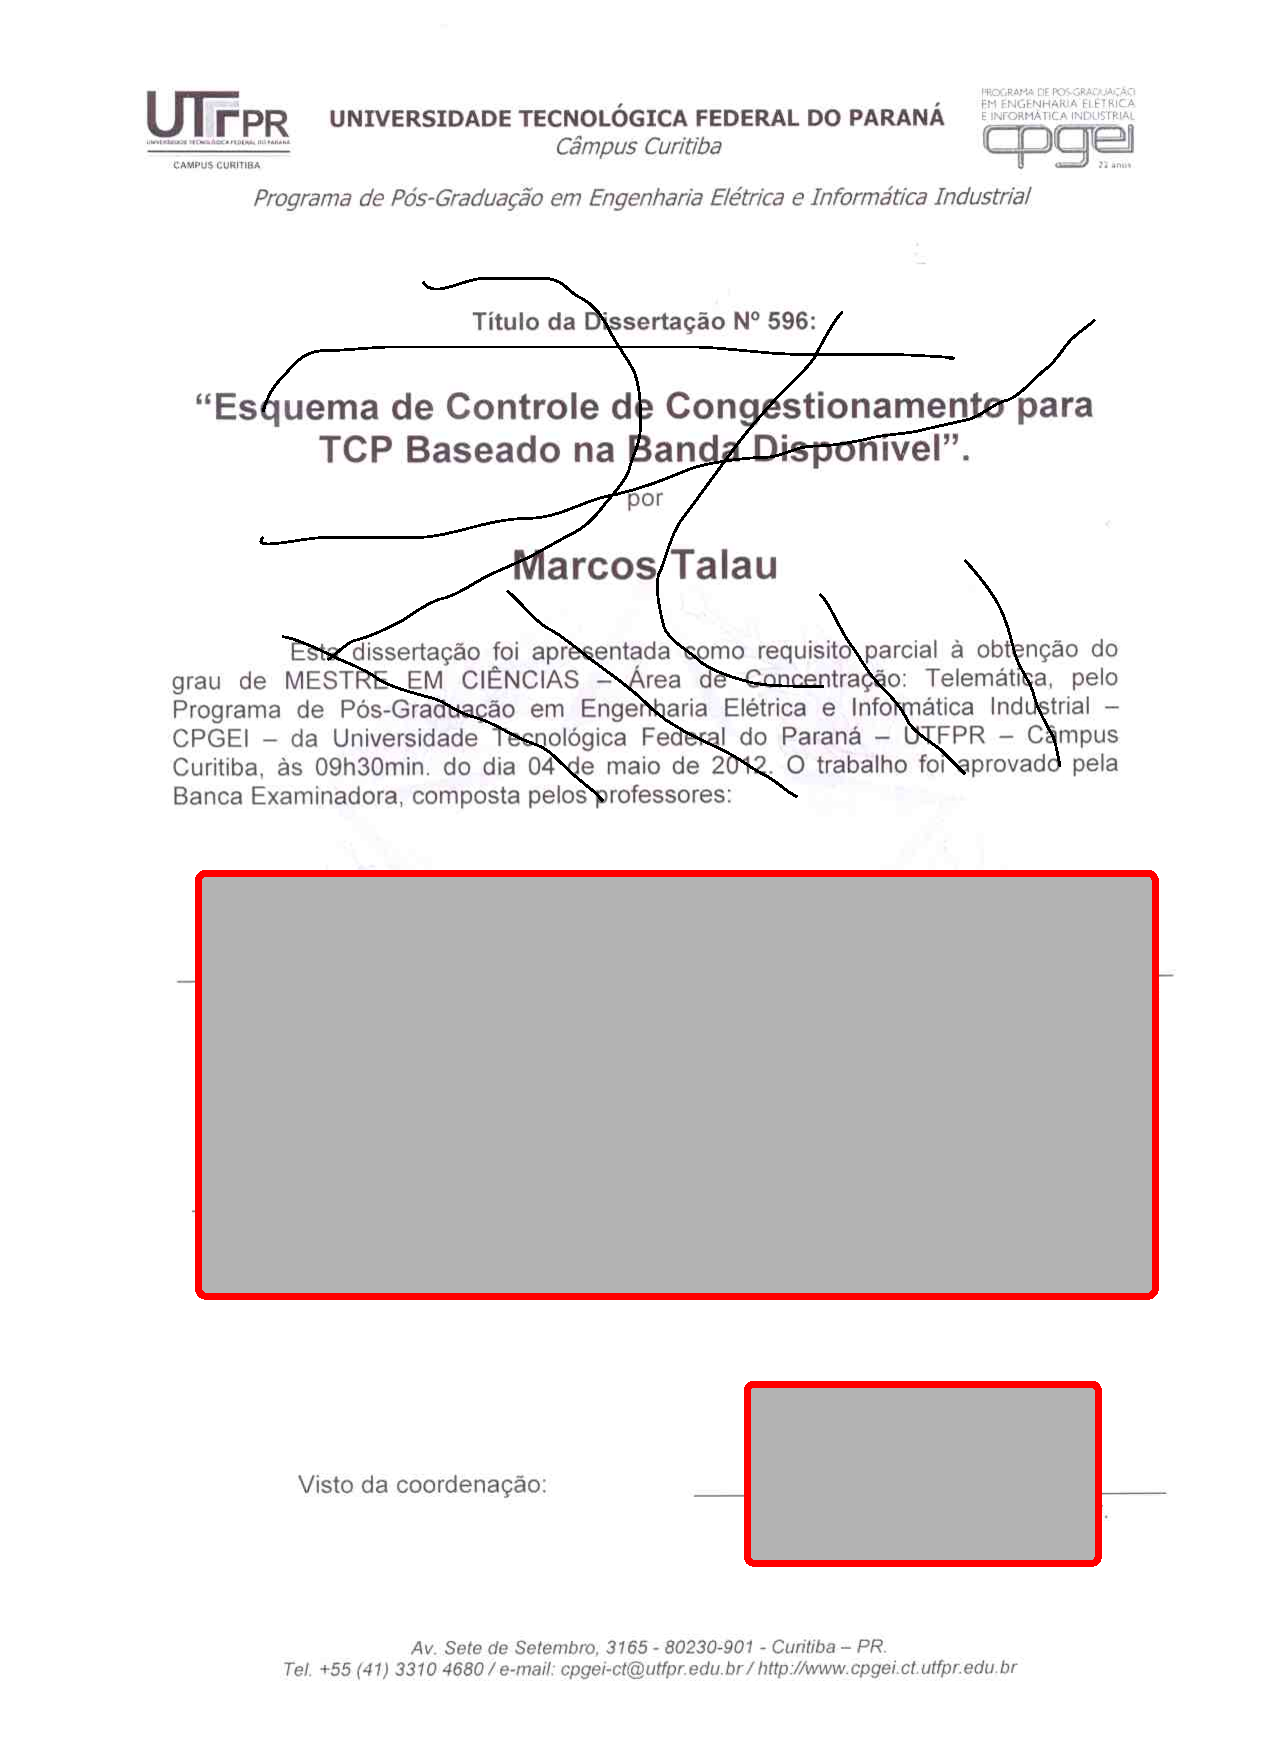
\includepdf{ata.pdf} %após a defesa scanear a ata e inserir o pdf na pasta raiz com o nome ata.pdf

%Caso utilize os itens dedicatória, agradecimentos ou epígrafe, lembar de retirar % antes do \include dos ou do item que for utilizar

% DEDICATÓRIA
\begin{dedicatoria}
 \vspace*{\fill}
 \noindent
  \raggedleft
 \begin{minipage}{.54\textwidth}
    Opcional
   \end{minipage}
\end{dedicatoria}


% AGRADECIMENTO
\begin{agradecimentos}

	Opcional


\end{agradecimentos}

%EPÍGRAFE
\begin{epigrafe}
    \vspace*{\fill}
	\begin{flushright}
	Opcional
	\end{flushright}
\end{epigrafe}

% RESUMO
% resumo em português
\begin{resumo}
\noindent
% Colocar o resumo entre a parte marcada
% Resumo aqui 
Nesta parte deve inserir o resumo do trabalho.

% Resumo até aqui
\end{resumo}

% resumo em inglês
\begin{abstract}
 \noindent 
% Colocar o resumo entre a parte marcada
% Abstract here 
Insert abstract here




% Abstract here	 
\end{abstract}

% listas (opcionais, mas recomenda-se a partir de 5 elementos)
\listadefiguras % geracao automatica da lista de figuras
%\listadetabelas % geracao automatica da lista de tabelas
\listadequadros % adivinhe :)
%\listadesiglas % geracao automatica da lista de siglas
\pagebreak
\begin{center}
\textbf{\MakeUppercase{Lista de Abreviaturas}}
\end{center}
\begin{acronym}[ASME]
\acro{ASME}[ASME] {American Society of Mechanical Engineers}
\acro{CAD}[CAD] {Computer-Aided Design}
\acro{DFA}[DFA] {Design for Assembly}
\acro{DFI}[DFI] {Design for Inspectability}
\acro{DFM}[DFM] {Design for Manufacturing}
\acro{DFMEA}[DFMEA] {Design Failure Mode and Effects Analysis}
\acro{DFR}[DFR] {Design for Recyclaibility}
\acro{DFS}[DFS] {Design for Serviceability}
\acro{DFX}[DFX] {Design for “X”}
\acro{DSR}[DSR] {Design Science Research}
\acro{GDT}[GD$\&$T] {Geometric Dimensioning and Tolerancing}
\acro{ISO}[ISO] {International Organization fo Standardization}
\acro{PDP}[PDP] {Processo de Desenvolvimento de Produto}
\acro{PMI}[PMI] {Product Manufacturing Information}
\acro{QI}[QI] {Qualidade de Informação}
\acro{VBA}[VBA] {Visual Basic for Applications}


\end{acronym}

%\listadesimbolos % geracao automatica da lista de simbolos

% sumario
\sumario % geracao automatica do sumario

%%%%%%%%%%%%%%%%%%%%%%%%%%%%%%%%%%%%%%%%%%%%%%%%%%%%%% ELEMENTOS TEXTUAIS
%%%%%%%%%%%%%%%%%%%%%%%%%%%%%%%%%%%%%%%%%%

\setcounter{page}{12}

% INTRODUÇÃO
\chapter{Introdução}

	\lipsum[1-1]

\section{Objetivo Geral}

	\lipsum[1-1]
\subsection{Objetivos Específicos}

	\lipsum[1-1]

\section{Justificativa}

\lipsum[1-1]
\section{Estrutura do Trabalho}

\lipsum[1-1]

%FUNDAMENTAÇÃO TEÓRICA
\chapter{FUNDAMENTAÇÃO TEÓRICA}
\lipsum[1-1]
\section{PROCESSO DE DESENVOLVIMENTO DE PRODUTOS E A INFORMAÇÃO}
\lipsum[1-5]








 








%ASPECTOS METODOLOGICOS
\chapter{ASPECTOS METODOLÓGICOS}
\label{ch:aspectosmetodologicos}
\lipsum[1-1]
\section{CARACTERIZAÇÃO DA PESQUISA}
\label{sec:caracterizacaodapesquisa}
\lipsum[1-1]
\section{ABORDAGEM METODOLÓGICA}
\label{sec:abordagemmetodologica}
\lipsum[1-1]
\section{PROCEDIMENTO METODOLÓGICO}
\label{sec:procedimentometodologico}
\lipsum[1-6]

%RESULTADOS
\newcommand*{\info}[4][25]{%
	\node [ annotation, #3, scale=.5, text width = #1cm,
	inner sep = 4mm ] at (#2) {%
		\list{$\bullet$}{\topsep=0pt\itemsep=0pt\parsep=0pt
			\parskip=2pt\labelwidth=6pt\leftmargin=6pt
			\itemindent=0pt\labelsep=2pt}%
		#4
		\endlist
	};
}
\chapter{Resultados e Discussão}
\label{ch:resultados}
\lipsum[1-12]

%CONCLUSÃO
\chapter{CONCLUSÃO}
\lipsum[1-1]

%%%%%%%%%%%%%%%%%%%%%%%%%%%%%%%%%%%%%%%%%%%%%%%%%%%%%% REFERENCIAS
%%%%%%%%%%%%%%%%%%%%%%%%%%%%%%%%%%%%%%%%%%

\clearpage % this is need for add +1 to pageref of bibstart used in 'ficha catalografica'.
\label{bibstart}
\bibliography{reflatex} % geracao automatica das referencias a partir do arquivo reflatex.bib ou substitua o arquivo com o nome de sua bibliteca .bib
\label{bibend}

%%%%%%%%%%%%%%%%%%%%%%%%%%%%%%%%%%%%%%%%%%%%%%%%%%%%%% ELEMENTOS POSTEXTUAIS
%%%%%%%%%%%%%%%%%%%%%%%%%%%%%%%%%%%%%%%%%%
%---------- Apendices (opcionais) ----------


\apendice
\chapter{Respostas dos Questionários}
\lipsum[1-1]


%Use o comando {\ttfamily \textbackslash apendice} e depois comandos {\ttfamily \textbackslash chapter\{\}}
%para gerar títulos de apêndices.





% ---------- Anexos (opcionais) ----------
\anexo

\chapter{Nome do Anexo}

\lipsum[1-1]





% --------- Ordenacao Afabetica da Lista de siglas --------
%\textbf{* Observa\c{c}\~oes:} a ordenacao alfabetica da lista de siglas ainda nao eh realizada de forma automatica, porem
% eh possivel se de realizar isto manualmente. Duas formas:
%
% ** Primeira forma)
%    A ordenacao eh feita com o auxilio do comando 'sort', disponivel em qualquer
% sistema Linux e UNIX, e tambem em sistemas Windows se instalado o coreutils (http://gnuwin32.sourceforge.net/packages/coreutils.htm)
% comandos para compilar e ordenar, supondo que seu arquivo se chame 'dissertacao.tex':
%
%      $ latex dissertacao
%      $ bibtex dissertacao && latex dissertacao
%      $ latex dissertacao
%      $ sort dissertacao.lsg > dissertacao.lsg.tmp
%      $ mv dissertacao.lsg.tmp dissertacao.lsg
%      $ latex dissertacao
%      $ dvipdf dissertacao.dvi
%
%
% ** Segunda forma)
%\textbf{Sugest\~ao:} crie outro arquivo .tex para siglas e utilize o comando \sigla{sigla}{descri\c{c}\~ao}.
%Para incluir este arquivo no final do arquivo, utilize o comando \input{arquivo.tex}.
%Assim, Todas as siglas serao geradas na ultima pagina. Entao, devera excluir a ultima pagina da versao final do arquivo
% PDF do seu documento.


%-------- Citacoes ---------
% - Utilize o comando \citeonline{...} para citacoes com o seguinte formato: Autor et al. (2011).
% Este tipo de formato eh utilizado no comeco do paragrafo. P.ex.: \citeonline{autor2011}

% - Utilize o comando \cite{...} para citacoeses no meio ou final do paragrafo. P.ex.: \cite{autor2011}



%-------- Titulos com nomes cientificos (titulo, capitulos e secoes) ----------
% Regra para escrita de nomes cientificos:
% Os nomes devem ser escritos em italico, 
%a primeira letra do primeiro nome deve ser em maiusculo e o restante em minusculo (inclusive a primeira letra do segundo nome).
% VEJA os exemplos abaixo.
% 
% 1) voce nao quer que a secao fique com uppercase (caixa alta) automaticamente:
%\section[nouppercase]{\MakeUppercase{Estudo dos efeitos da radiacao ultravioleta C e TFD em celulas de} {\textit{Saccharomyces boulardii}}
%
% 2) por padrao os cases (maiusculas/minuscula) sao ajustados automaticamente, voce nao precisa usar makeuppercase e afins.
% \section{Introducao} % a introducao sera posta no texto como INTRODUCAO, automaticamente, como a norma indica.


\end{document}

